\section{Arbeitsablauf des Schlussfolgerers}

In der nachfolgenden Abbildung \ref{image-u2r3-workflow} ist der gewöhnliche Ablauf des Reasoner dargestellt. Dabei ist er in dreih Phasen einzuteilen. Das LAden der Ontologie, der Schlussfolgerungsvorgang und die Abfrage .

\begin{figure}
	\caption{Arbeitsablauf des Schlussfolgerers}
	\label{image-u2r3-workflow}
	\scalebox{0.6}{
		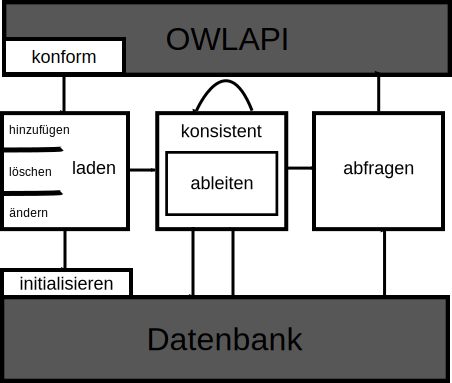
\includegraphics{images/u2r3-workflow.pdf}
	}
\end{figure}

konform: überprüft, ob die verwendete Syntax im OWL2 RL Profil liegt
laden: bringt die Ontolgoie in das Datenbank-Schema, dabei merkt es an welche Regeln für das ableiten ausgeführt werden sollen
initialisieren: erzeugt das Datenbankschema notfalls, läd Standardwerte und richtet in der Datenbank nötige Funktionen ein
konsistent: ist eine Hülle um dafür zu sorgen, das nur über konsistente Fakten geschlossen wird. Die Häufigkeit kann eingestellt werden.
ableiten:Wendet die Ableitungsregeln an. Die Regelandwendung ist abgschloßen wenn keine neuen Fakten erzeugt werden können.
abfragen: implementiert die Schnittstelle der OWLAPI, mit der man Anfragen an die abgeleiteten Fakten stellen kann

OWLAPI Anbindung

Der obere Teil ist die sogenannte OWLAPI. Die OWLAPI ist eine Bibliothek die das Auslesen von Ontologien in verschiedenen Formaten erlaubt und eine Schlussfolgererschnittstelle für andere Programme zur Verfügung stellt. Durch die Implementierung dieser Schnittstelle in U2R3 ist es für alle Programme zugänglich die mit der OWLAPI arbeiten.
Die Schnittstelle stellt dabei auch eine Liste typischer Abfragen für einen Reasoner dar und kann allein dadurch schon als Messlatte für die Fähigkeiten eines Schlussfolgerers verwendet werden. Das OWLAPI-Projekt ist open-source und in Java implementiert und ist damit auch optimal für die Implementierung von U2R3 geeignet. Neben der reinen Parsertätigkeit kann die OWLAPI auch noch helfen zu überprüfen, ob eine Ontologie im OWL2 RL Profil liegt und nimmt damit weitere Arbeit ab.

\subsection{Das Laden einer Ontologie}

Die Inhalte einer Ontolgie die für das Schlussfolgern wichtig sind, sind die Axiome. Axiome sind dabei Fakten die als allgemein gültig angenommen werden. Sie dienen dazu das Universum der Ontologie zu modellieren und einen Startpunkt für weitere Schlussfolgerungen zu erzeugen.

Alle Axiome werden entsprechend dem MEMA-Prinzip abgelegt. Dabei ist für jedes Axiom genau eine Relation vorgesehen. Falls die Ontologie nicht OWL2 RL konform ist müssen für gewisse Axiome implizite Informationen abgelegt, wie. z.B.

\begin{table}
	\begin{tabular}{|l|l|}
    \hline
    If & then \\
    \hline
	T(?i1, ?property, ?i2 & property owl:type ObjectProperty \\
	\hline
    \end{tabular}
\end{table}


\begin{verbatim}
* Wie wandelt man die Ontologie in INSERTs um?
* Wie läd man eine Ontologie?
\end{verbatim}


Falls ein Axiom aus komplexen Ausdrücken zusammengesetzt ist werden die Ausdrücke rekursiv abgearbeitet und einzeln behandelt. Zum herstellen der Beziehungen bei komplexen Axiomen werden Platzhalter für die Ausdrücke verwendet. Die Platzhalter die dabei erzeugt werden stammen von der OWLAPI aus der NodeID Klasse und folgen damit dem selben Schema wie auch bei anonymen Individuen.

Bsp:
\begin{verbatim}
(A int (Svf p B)) subC C
      nid1             C    subClass(nid1, C)
      nic2                  intOf(nid1, nid2)
 A         nid3             list(nid2, A, nid3)
            p B             svf(nid3, p, B)
\end{verbatim}

Wenn Fakten in eine Relation geschrieben werden, wird von dieser ein Hinweis (\emph{Reason}) an den Regelprozessor geschickt.

Dieser überprüft die Ursache und legt entsprechende Regeln an, die auf diese Veränderung ausgeführt werden können.

Die abzuarbeitenden Regeln enthalten eine Referenz auf die Fakten, die hinzugekommen sind. Allgemein sind sie so implementiert, das sie nur auf diesen neuen Fakten arbeiten -  auf den sogenannten Deltas - dies ist allerdings nicht in allen Fällen möglich (\emph{cls-int1}), sinnvoll (zu viele verschiedene Kombinationsmöglichkeiten) oder einfach zu komplex und damit fehleranfällig (\emph{prp-spo2}). Falls zwei oder mehrmals eine Regel auf die selben neuen Fakten erzeugt wird bevor sie ausgelöst wird, werden die beiden Regeln zu einer zusammengefasst und können je nach Einstellung neu priorisiert werden.

All diese Regeln sind in einer Warteschleife abgelegt, die beim laden der Ontologie gefüllt wird und beim abarbeiten, d.h. dem realisieren, der Ontologie ausgelesen wird.

Regeln können durch das Erzeugen von neuen Fakten Hinweise für den Regelprozessor geben der daraufhin weitere Regeln anlegt und in die Warteschlange einsortiert.

Der Vorgang des Realisierens ist abgeschlossen, wenn keine Regel neue Fakten und damit neue Regeln erzeugen kann.

Der OWL2 RL Regelsatz garantiert dabei, das es immer zu einem Ende der Regelanwendung kommen wird, egal ob eine gültige oder ungültige Ontologie geladen wird.

Für das Abarbeiten und Erzeugen der Regeln ist hauptsächlich der Regelprozessor verantwortlich. Hier sind noch weitere Einstellungsmöglichkeiten, wie z.B. die parallele Verarbeitung von Regeln vorhanden.


\subsection{Das Schlussfolgern in einer Ontologie}

\subsection{Das Abfragen einer Ontologie}


